\documentclass[
	%parspace, % Add vertical space between paragraphs
	%noindent, % No indentation of first lines in each paragraph
	%nohyp, % No hyphenation of words
	%twoside, % Double sided format
	%draft, % Quicker draft compilation without rendering images
	%final, % Set final to hide todos
]{nemeth_zsofia_reka_elte_ik_thesis}[2025/03/17]

% The minted package is also supported for source highlighting
% See elteikthesis_minted.tex for example
%\usepackage[newfloat]{minted}

% Document's metadata
\title{Pénzügyeket rendszerező webes alkalmazás} % title
\date{2025} % year of defense

% Author's metadata
\author{Németh Zsófia Réka}
\degree{programtervező informatikus BSc}

% Superivsor(s)' metadata
\supervisor{Dr. Bende Imre} % internal supervisor's name
\affiliation{egyetemi adjunktus} % internal supervisor's affiliation
%\extsupervisor{Külső Kornél} % external supervisor's name
%\extaffiliation{informatikai igazgató} % external supervisor's affiliation

% University's metadata
\university{Eötvös Loránd Tudományegyetem} % university's name
\faculty{Informatikai Kar} % faculty's name
\department{Média- és Oktatásinformatika Tanszék} % department's name
\city{Budapest} % city
\logo{elte_cimer_szines} % logo

% Add bibliography file
\addbibresource{elteikthesis.bib}

% The document
\begin{document}

% Set document language
\documentlang{hungarian}
%\documentlang{english}

% List of todos (not in the final document)
%\listoftodos[\todolabel]

% Title page (mandatory)
\maketitle
% Topic declaration page (mandatory) - can also be attached instead
%\includepdf{temabejelento.pdf}

% Table of contents (mandatory)
\tableofcontents
\cleardoublepage

% Main content
\chapter{Bevezetés}
\label{ch:intro}

A választott témám egy személyes pénzügyeket rendszerező webalkalmazás. A dolgozat a full-stack webfejlesztés témaköréhez kapcsolódik, mivel frontend-, backend- és adatbáziskezelést is magában foglal. A backendet és a frontendet egy projekt részeként, egy C\# alapú ASP.NET Web App (Razor Pages) (.NET 8) keretrendszerrel valósítottam meg, amelyhez egy MySQL relációs adatbázist csatoltam az Entity Framework segítségével. A .NET lehetőséget nyújt különböző frontend keretrendszerek használatára is, azonban a webalkalmazásomat jelenleg egy egyszerű HTML/CSS/JavaScript kombináció alkotja, Bootstrap (CSS framework) elemek felhasználásával.

Az alkalmazás fő lényege, hogy a felhasználó költéseit és bevételeit nyomon tudja követni, megtakarításait kezelhesse akár egyénileg, akár csoportokban, mindezt egy felhasználóbarát felületen. Az alkalmazás az alap funkciókon kívül még kimutatásokat is készít a felhasználó pénzkezelési szokásairól, melyeket akár PDF formátumban is le lehet tölteni.


Véleményem szerint a már erre a célre létrehozott megoldások egy része túlságosan leegyszerűsített, másik része pedig annyira összetett és funkciógazdag, hogy hétköznapi felhasználók számára nehezen átláthatóvá válik. Jelen alkalmazás ezt az ellentétet próbálja kiegyensúlyozni, egy egyszerű, de funkcionális megoldást kínálva.


A következő fejezetekben részletesen bemutatom a projektet a felhasználói és fejlesztői dokumentációkon keresztül.

\cleardoublepage

\chapter{Felhasználói dokumentáció}
\label{ch:user}

A következő fejezetben fogom bemutatni az alkalmazás elérését, egyes komponenseit, illetve felhasználási lehetőségeit. 

Ez a pénzügyeket rendszerező alkalmazás alapvetően magánszemélyeknek készült, személyes felhasználásra, de mivel lehetőséget nyújt csoportos használatra is, ezáltal akár egy kisebb vállalat igényeit is elláthatja.

A főbb funkciók közé tartozik, hogy bevételeket és kiadásokat lehet rögzíteni, kategóriák szerint csoportosítva, illetve kimutatásokat nézhet a felhasználó a pénzügyi szokásairól, melyeket exportálni is tudja. Az alkalmazás egyik nagy előnye, hogy nem csak egyének használhatják, hanem csoportok (például háztartások) is.


\section{Rendszerkövetelmények}

Mivel egy webes alkalmazásról van szó, ezért különleges gépigény nem szükséges. Szinte az összes böngésző támogatott.

\section{Felhasználói esetek}

Az alkalmazás felhasználói eseteit ez a bejegyzés fogja taglalni jobban, képernyőképekkel magyarázva.
\begin{table}[H]
	\centering
	\begin{tabular}{ | m{0.25\textwidth} | m{0.65\textwidth} | }
		\hline
		\textbf{Funkció} & \textbf{Leírás} \\
		\hline \hline
		\emph{Bejelentkezés} & Bejelentkezés egy egyedi felhasználónévvel és egy jelszóval lehetséges \\
		\hline
		\emph{Regisztráció} &  Quisque lobortis eros vitae urna lacinia euismod. \\
		\hline
		\emph{Elfelejtett jelszó} & Curabitur ac lacus pellentesque, eleifend sem ut, placerat enim. Ut auctor tempor odio ut dapibus. \\
		\hline
	\end{tabular}
	\caption{Maecenas tincidunt non justo quis accumsan}
	\label{tab:example-1}
\end{table}

\begin{figure}[H]
	\centering
	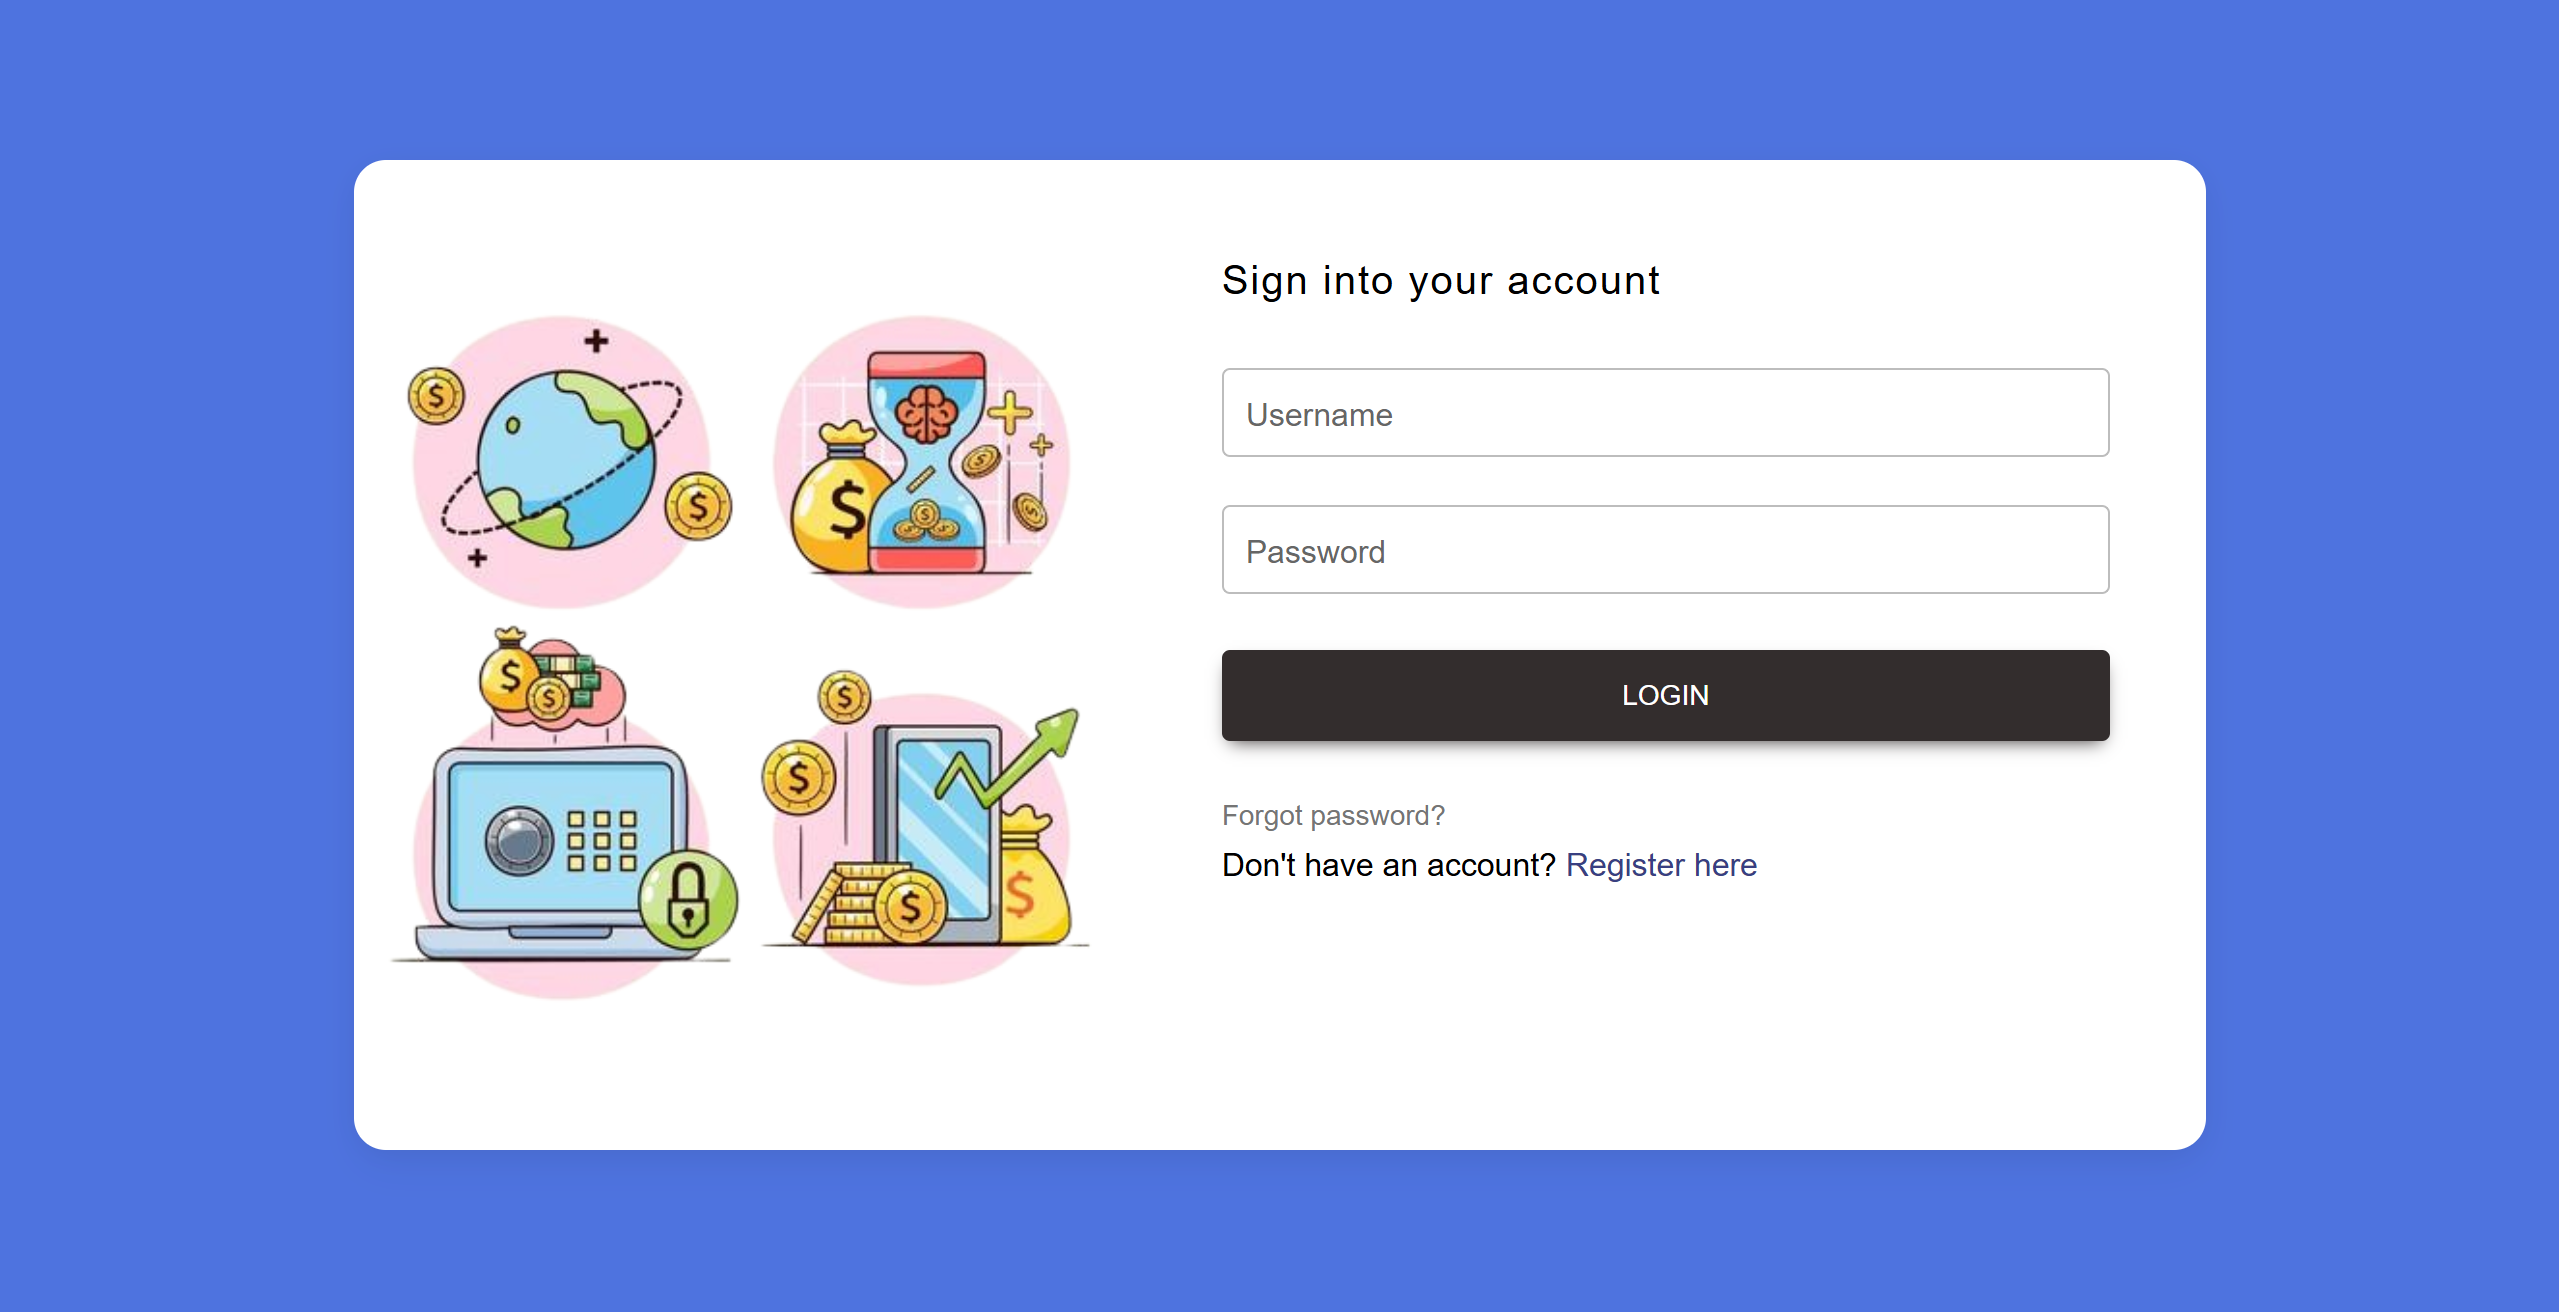
\includegraphics[height=180px]{img/login-screenshot}
	\caption{Screenshot: Bejelentkező felület}
	\label{fig:example-1}
\end{figure}

\cleardoublepage

\chapter{Fejlesztői dokumentáció}
\label{ch:impl}
 A következő fejezetben az alkalmazást fejlesztői szemszögből mutatom be. Részletesen kitérek az alkalmazás felépítésére, a használt technológiákra, az adatbázis-struktúrára, valamint a fejlesztés során követett elvekre és megoldásokra.

\section{Architektúra}
\begin{itemize}
	\item Frontend: HTML\footnote{Mivel a C\# projekten
		belül lett létrehozva a frontend is, ezért a .html helyett .cshtml
		kiterjesztésű fájlok vannak. Ezek annyiban különböznek a 
		HTML-től, hogy vannak bizonyos tagek, kulcsszavak, melyekkel
		különleges dolgokat tudunk csinálni. A Frontend című fejezetben kerül ez a téma bővebb kifejtésre.}/CSS/JavaScript (és Bootstrap)
	\item Backend: C\# (ASP.NET Web App (Razor Pages))
	\item Adatbázis: MySQL relációs adatbázis
\end{itemize}

\begin{figure}[H]
	\centering
	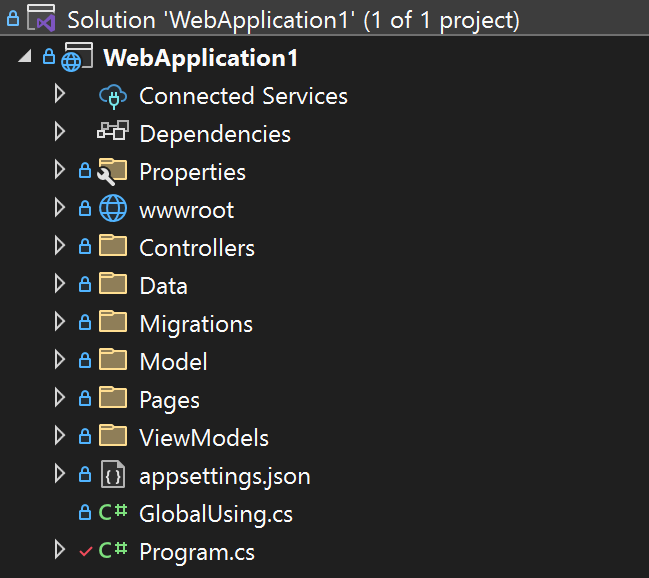
\includegraphics[height=220px]{img/solution-explorer-screenshot}
	\caption{Projekt struktúra}
	\label{fig:project-structure}
\end{figure}

\subsection{Külső függőségek, technológiák}

Csomagok hozzáadása a projekthez történhet a NuGet Package Manager vagy CDN segítségével is. Az alkalmazás fejlesztése során az alábbi külső csomagok és könyvtárak kerültek felhasználásra:

\begin{itemize}
	\item \textbf{Entity Framework Core (EF Core)} – ORM technológia, amely lehetővé teszi az adatbázissal való objektumorientált munkát. Kiemelten hasznos a LINQ támogatása és a migrációs rendszer.\footnote{A migrációk működéséről az adatbázissal foglalkozó fejezet fog részletesebb leírást nyújtani.}
	\item \textbf{Pomelo.EntityFrameworkCore.MySql} – Az EF Core és a MySQL adatbázis közötti kapcsolatot biztosító NuGet csomag.
	\item \textbf{MySqlConnector} – Könnyűsúlyú, aszinkron támogatással rendelkező ADO.NET driver MySQL-hez.
	\item \textbf{Swashbuckle.AspNetCore} – A Swagger UI integrálására szolgáló csomag, amely lehetővé teszi az API-k dokumentálását és tesztelését.
	\item \textbf{Bootstrap} – Reszponzív front-end keretrendszer, amely előre definiált CSS osztályokat és JavaScript komponenseket biztosít a felhasználói felület egységes és gyors kialakításához. Az alkalmazás a Bootstrap 4-es verzióját használja, amely lehetővé teszi különböző vizuális elemek (például gombok, táblázatok, rácsszerkezetek) egyszerű alkalmazását csupán megfelelő class attribútumok beállításával. Nem csak az esztétikus megjelenésben nyújt segítséget a Bootstraom hanem interaktív viselkedések (pl. modális ablakok, lenyíló menük) hozzáadásában is, beépített JavaScript funkciók segítségével.
	\item \textbf{FontAwesome (CDN)} – Ikonok használatához alkalmazott ikoncsomag.
	\item \textbf{QuestPDF} -Az alkalmazás lehetőséget nyújt az adatok exportálására nyomtatható formátumban, egy PDF fájl formájában. Erre a célra a QuestPDF nevű nyílt forráskódú .NET könyvtárat használtam.
	
	A QuestPDF lehetővé teszi professzionális minőségű PDF fájlok generálását teljes mértékben C\# nyelvben, deklaratív stílusban. Előnyei:
	\begin{itemize}
		\item Reszponzív dokumentumelrendezés
		\item Könnyen tanulható, C\#-os fluent API
		\item Támogatja a táblázatokat, stílusokat, színeket, képeket
	\end{itemize}

A generálás egy `Document.Create(...)` hívással történik, ahol meghatározásra kerül a dokumentum szerkezete, stílusa, tartalma. Például:
	
	\lstset{caption={PDF generálás példa}, label=src:pdf}
	\begin{lstlisting}[language={[Sharp]C}]
		Document.Create(container =>
		{
			container.Page(page =>
			{
				page.Content()
				.Column(col =>
				{
					col.Item().Text("Kiadasi osszesito");
					col.Item().Text("Osszes tranzakcio: 42");
				});
			});
		}).GeneratePdf("output.pdf");
	\end{lstlisting}
	
	A PDF fájl generálása szerveroldalon történik, a Utils/PDFGenerator.cs osztályban megvalósított logika segítségével. A kész fájl ezután egy HTTP végpont (Controller) segítségével érhető el és tölthető le a felhasználó által.
	
	\lstset{caption={PDF generálás API végpont}, label=src:pdf}
	\begin{lstlisting}[language={[Sharp]C}]
		[HttpGet("DownloadReportForCurrent")]
		public async Task<IActionResult> DownloadReport()
		{
			// get data
			
			var pdf = new PdfGenerator(user.Fullname, transactions);
			var pdfBytes = pdf.GeneratePdf();
			
			return File(pdfBytes, "application/pdf", $"report_{user.Fullname}_{DateTime.Now:yyyyMMdd}.pdf");
		}
	\end{lstlisting}
	\item \textbf{Chart.js} – Az alkalmazás az adatok vizuális megjelenítésére a népszerű JavaScript könyvtárat használja, amely interaktív, reszponzív grafikonokat képes kirajzolni HTML canvas elemeken keresztül.
	
	Két típusú diagram került megvalósításra, melyek közül az utóbbi csoportokban nem elérhető:
	\begin{itemize}
		\item Napi bontású bevétel és kiadás alakulása az aktuális hónapban (vonaldiagram)
		\item Havi bontású bevétel–kiadás összehasonlító diagram (oszlopdiagram)
	\end{itemize}
	
	A grafikonok kliensoldalon, JavaScript segítségével jönnek létre. Az adatok aszinkron módon kerülnek lekérésre az API végpontokról, a felhasználó azonosítója alapján. A lekért tranzakciós adatok formázása és csoportosítása után a rendszer automatikusan diagramot generál azok vizuális megjelenítésére.
	
	Az alábbi példában látható egy egyszerűbb diagram kirajzolása:
	
	\lstset{caption={Chart.js alapú havi diagram kirajzolása}, label=src:chartjs}
	\begin{lstlisting}[language={[Sharp]C}]
 	const ctx = document.getElementById("finance-chart");
 	// <canvas> elem
 	const monthlySpendingChart = new Chart(ctx, {
 		type: 'bar',
 		data: {
 			labels: months, // Jan - Dec
 			datasets: [{
 				label: "Income",
 				data: incomeData // from backend
 			}]
 		}
 	});
	\end{lstlisting}
\end{itemize}

\subsection{Architektúra leírása}
Ahogy a \ref{fig:project-structure}. ábrán is látható, az egész webalkalmazás egy projekten belül lett kialakítva. A .NET-es integrált frontend és backend fejlesztés hatalmas előnye a rendszerezettség, a szabályszerű kommunikáció az egyes rétegek között (illetve ezen rétegek helyes elkülönölése), és a rengeteg beépített segédfüggvény/konfiguráció/cshtml tag. Kiemelném még a modellek használatát is, amelyek egyszerűbb és biztonságosabb (például SQL injection elleni védelem) adatbázis kezelést biztosítanak.

Az egyes route-ok konfigurálása is meglehetősen letisztult ebben a keretrendszerben. A "Pages" mappa\footnote{A "Pages" mappa, ahogy a neve is mutatja, tartalmazza a weboldal egyes oldalait. Bővebb kifejtés a Frontend című fejezetben.} fájlstruktúrája alapján automatikusan létrejönnek a route-ok, ha a "Program.cs"-ben megadjuk a programnak, hogy hozza létre őket:

\lstset{caption={Route-ok konfigurálása}, label=src:routing}
\begin{lstlisting}[language={[Sharp]C}]
	app.UseRouting();
\end{lstlisting}

A frontend és a backend közötti hagyományos JavaScript segítségével történő kommunikáción kívül, a cshtml formátum miatt lehetőség nyílik egyszerűbb esetekre közvetlen kapcsolatot is létesíteni a backend és a frontend között. Például:

\lstset{caption={Frontend modell egy alkalmazása}, label=src:model}
\begin{lstlisting}[language={HTML}]
	<h1>Username</h1>
	<p>@Model.UserData.Username</p>
\end{lstlisting}

Itt ugye mint látható a modellből tudunk adatot lekérdezni.
De mi is a "Model" pontosan? Ugyebár az ASP .NET Web App keretrendszer úgy működik, hogy minden oldal (Razor page) egy .cshtml és egy .cs fájl együtteséből áll össze. A .cs kiterjesztésű fájl az adott oldal modellje. Itt definiálhatunk adatszerkezeteket és függvényeket, mint például az OnGet() és OnPost(), amelyek beépített (opcionális) metódusok, és ahogy a nevük is mutatja,
az oldalról érkező GET és POST requesteket kezelik. Tehát például,
ha az adott oldalon egy darab form-unk van, amit POST metódussal
be akarunk küldeni a szervernek, ezt JS (JavaScript) kód írása nélkül biztonságosan meg tudjuk tenni.

\section{Frontend}
Térjünk át a frontend réteg alkotóelemeire, és ezek működésére. Itt is komponensenként fogom bemutatni a felhasznált technológiákat.
\begin{figure}[H]
	\centering
	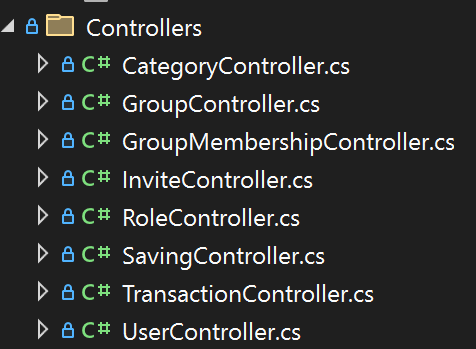
\includegraphics[height=140px]{img/controllers}
	\caption{Pages struktúra}
	\label{fig:controllers}
\end{figure}
\subsection{Layout}
A "Pages" mappa tartalmazza az oldalakat. A keretrendszer ugyebár úgy működik, hogy minden oldal (Razor page) egy .cshtml és egy .cs
fájl együtteséből áll össze. A Pages mappa ezeket a párosokat tartalmazza, további kisebb mappákra bontva a funkció csoportok alapján. Az alább mellékelt ábrából (\ref{fig:pages-structure}. ábra) látható tehát, hogy például a bejelentkező felületet a következő linken tudjuk elérni: "localhost:<<port>>/Account/Login".

\begin{figure}[H]
	\centering
	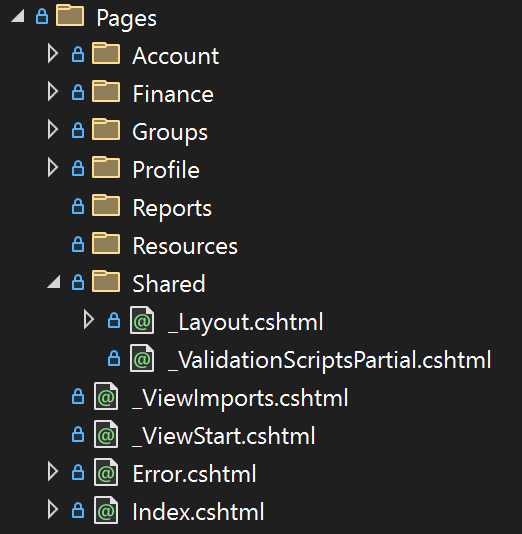
\includegraphics[height=240px]{img/solution-explorer-pages-screenshot}
	\caption{Pages struktúra}
	\label{fig:pages-structure}
\end{figure}

Találhatók még ebben a mappában egyéb segédfájlok is, mint például az Error.cshtml, ami az esetleges hibák esetén jelenik meg. Kiemelendő még a Shared mappa, amiben található egy Layout.cshtml fájl is (modell nélkül). Ez, ahogy a neve is mutatja egy alap sablont biztosít az alkalmazás felületének. A weboldal egy (a képernyő baloldán lévő) főmenüből, egy kis (az oldal tetején található) menüsávból, a fő tartalmi részből áll, illetve egy footer részből áll. A footer és a menüsávok kódját tartalmazza a Layout.cshtml között a tartalomnak "kihagyott" rész: 
\lstset{caption={Layout extension ASP.NET keretrendszerben}, label=src:csharp}
\begin{lstlisting}[language={HTML}]
	<div class="container-fluid">
	@RenderBody()
	</div>
\end{lstlisting}

A RenderBody() függvény (szintén beépített .NET metódus)
behelyezi az adott oldal HTML kódját ebbe a div HTML elembe. Ez
automatikusan megtörténik az összes oldal esetében amelyre
navigál a felhasználó. Ha valami miatt éppen nem ezt a sablont akarjuk követni egy oldalunkkal (például: Bejelentkező felület), akkor az adott oldal HTML kódjába beírhatjuk hogy ne sablont kövessen:

\begin{lstlisting}[language={[Sharp]C}]
	@{
		Layout = null; // Remove layout if you want a standalone page
	}
\end{lstlisting}

\subsection{Statikus erőforrások kezelése}

A \texttt{wwwroot} mappa szolgál az alkalmazás összes statikus erőforrásának (static resources) tárolására. Ide kerülnek azok a fájlok, amelyeket a kliensoldal közvetlenül elérhet, például JavaScript állományok, CSS (stílus formázás) fájlok, képek vagy betűtípusok. A mappa struktúráját (a szokásokhoz híven) a következőképpen alakítottam ki:

\begin{itemize}
	\item \texttt{js} – JavaScript fájlok
	\item \texttt{css} – CSS fájlok
	\item \texttt{img} – Képek (ikonok, háttérképek stb.)
\end{itemize}

Az alkalmazás formázásához a Bootstrap keretrendszer 4-es verzióját használtam. A Bootstrap szükséges CSS és JavaScript fájljait közvetlenül letöltve helyeztem el a \texttt{wwwroot} mappában, így külső CDN-től való függőség nélkül működik az alkalmazás. Egyetlen kivételt képez egy betűtípus, amely CDN-en keresztül kerül betöltésre.

A \texttt{wwwroot} mappában elhelyezett fájlok az alkalmazás nézeteiből (\texttt{.cshtml} fájlokból) egyszerűen beilleszthetők az alábbi módon:

\begin{lstlisting}[language=HTML, caption={Statikus fájlok hivatkozása .cshtml fájlban}]
	<link rel="stylesheet" href="~/css/style.css" />
	<script src="~/js/site.js"></script>
\end{lstlisting}

A "\~{}" jelölés a gyökérmappára hivatkozik, így biztosítva a helyes útvonalat (minden környezetben).

\section{Backend}

A következő fejezetben az alkalmazás backend architektúráját mutatom be, kifejtve az egyes elemek funkcióit és használatát.

\subsection{appsettings.json}

Az appsettings.json egy konfigurációs
fájl. Ebben lehet alkalmazásszintű beállításokat tárolni, például:
adatbáziskapcsolati stringeket,
API kulcsokat,
logolási beállításokat,
vagy bármilyen egyedi, fejlesztő által definiált értéket.
Az értékeket a program bármely részén könnyen ki lehet olvasni (szótár szintaktika használatával)  (pl. Configuration["Kulcs"]). Ez segít elkülöníteni a kódot a
konfigurációtól, így könnyebb a karbantartás, és egyszerűen kezelhető a környezetenkénti
eltérés (pl. fejlesztői vs. éles környezet).

\subsection{Program.cs}
Ez a fő program fájl, és egyben az alkalmazás belépési pontja. Ebben készítjük
elő a webalkalmazásunk tulajdonságait (persze a Razor Pages egyszerűségének
hála ez nem sok plusz feladattal jár, csupán a helyes függvényeket
kell meghívni helyes sorrendben, attól függően, hogy hogyan
akarjuk konfigurálni az alkalmazást). Itt lehet beállítani a
korábban említett routing-ot, az autentikációt, a cookie-kat,
a session-t, a fejlesztői és éles környezeteket, és még sok minden mást. Itt tudjuk felkonfigurálni a modellt, az adatbázist
és az oldalakat (Pages) is. ezután az app.Run() függvény hívással
tudjuk ténylegesen elindítani a weboldalt.

\subsection{Modellek}
Minden adatbázis táblának létrehozunk egy modellt
(bővebb kifejtés az "adatbázis" pontban). Ezek mind C\# osztályok
táblánként, és minden oszlop egy külön propertynek feleltethető meg.

Az alkalmazásban minden adatbázis tábla egy hozzá tartozó C\# osztállyal, azaz modellel van leképezve. Ezek az osztályok tartalmazzák az adott tábla mezőit, mint property-ket, valamint opcionálisan kapcsolatok (navigációs tulajdonságok) is definiálhatók a táblák között, például egy tranzakcióhoz tartozó felhasználó vagy kategória esetén.

A modellek létrehozása kulcsfontosságú az Entity Framework Core működéséhez, mivel ezek alapján tudja az ORM keretrendszer leképezni az adatbázis szerkezetét, valamint automatikusan kezelni a lekérdezéseket, beszúrásokat és módosításokat. A modellek az \texttt{ApplicationDbContext} osztályban kerülnek regisztrálásra, amely az adatbázis-kapcsolatot is kezeli.

Például egy egyszerű \texttt{Transaction} modell így nézhet ki:

\begin{lstlisting}[language={[Sharp]C}, caption={Egyszerű modell osztály példa}]
	public class Transaction
	{
		public int Id { get; set; }
		public int UserId { get; set; }
		public decimal Amount { get; set; }
		public DateTime Date { get; set; }
		public string Description { get; set; }
	}
\end{lstlisting}


\subsection{API-kezelés és végpontok kialakítása}

Az ASP.NET alkalmazás szerkezete lehetővé teszi, hogy a frontend és a backend között tisztán elválasztott, jól strukturált kommunikáció jöjjön létre. Miután a \texttt{Program.cs} fájlban megtörténik a szükséges szolgáltatások regisztrálása és konfigurációja (pl. routing, dependency injection), a fejlesztés következő lépése az API-végpontok kialakítása.

Az alkalmazás \texttt{Controllers} mappájában (\ref{fig:controllers}.~ábra) minden releváns adatmodellhez külön kontrollerosztály tartozik, ahol HTTP-alapú végpontokat definiálok (pl. \texttt{GET}, \texttt{POST}, \texttt{PUT}, \texttt{DELETE} metódusok). Ezeket a végpontokat a frontend JavaScript kód hívja meg aszinkron módon \texttt{fetch} API segítségével, ezáltal biztosítva a felhasználó és a szerver közötti kétirányú adatkommunikációt.

Az egyszerűbb esetekben (például egy adatmodell értékeinek megjelenítése) az ASP.NET Razor Pages lehetőséget biztosít arra, hogy közvetlenül a \texttt{.cshtml} nézetfájlban jelenítsünk meg backendből érkező adatokat a modellobjektumok segítségével. Az összetettebb működések (pl. szűrés, exportálás, állapotváltoztatás) viszont külön API-végpontokat igényelnek.

A fejlesztés során az API-dokumentáció és tesztelés megkönnyítésére a \textbf{Swagger} (Swashbuckle.AspNetCore) könyvtár került integrálásra. Ez automatikusan generál egy böngészőben elérhető dokumentációs felületet, ahol a végpontok struktúrája, paraméterei és válaszai is megtekinthetők, valamint tesztelhetők. Fontos biztonsági szempont, hogy a Swagger csak \texttt{Development} környezetben legyen elérhető, nehogy érzékeny információk szivárogjanak ki az éles rendszerből.
\subsubsection{Példa API Controller}

Az alábbi kódrészlet bemutatja, hogyan történik egy egyszerű \texttt{GET} kérés kezelése, amely egy adott felhasználóhoz tartozó tranzakciókat ad vissza.

\lstset{caption={Egyszerű Controller példa – tranzakciók lekérdezése}, label=src:controller}
\begin{lstlisting}[language={[Sharp]C}]
	[ApiController]
	[Route("api/[controller]")]
	public class TransactionController : ControllerBase
	{
		private readonly ApplicationDbContext _context;
		
		public TransactionController(ApplicationDbContext context)
		{
			_context = context;
		}
		
		// GET: api/Transaction/user/5/type/1
		[HttpGet("user/{userId}/type/{typeId}")]
		public IActionResult GetTransactionsByUserAndType(int userId, int typeId)
		{
			var transactions = _context.Transactions
			.Where(t => t.UserId == userId && t.TypeId == typeId)
			.OrderByDescending(t => t.Date)
			.ToList();
			
			return Ok(transactions);
		}
	}
\end{lstlisting}

A fenti példában a kontroller egy adott felhasználó és tranzakciótípus alapján szűri az adatokat, majd egy JSON-formátumú listát ad vissza, amit a frontend JavaScript-kód aszinkron módon feldolgoz. Ez az endpoint tehát tökéletesen alkalmas például diagramok vagy riportok adatainak kiszolgálására.

\section{Adatbázis}
Az alkalmazás működésének egyik alapvető pillére az adatbázis, amely a rendszerben tárolt információk strukturált kezelését, hosszú távú perzisztenciáját és elérhetőségét biztosítja. Az adatbázis szerkezete úgy került kialakításra, hogy az hatékonyan támogassa az alkalmazás funkcionális igényeit, miközben jól skálázható és könnyen karbantartható maradjon.

Az adatbázis relációs modellre épül, és az adatok külön táblákban kerülnek tárolásra, melyeket kulcsok és kapcsolat típusok kötnek össze.

\subsection{Szerkezet}
Az alkalmazás adatbázisa egy localhost-on futó MySQL adatbázis.
A MySQL sok szempont miatt kiváló választás kisebb alkalmazásokhoz, ezek közé tartozik például az a nem elhanyagolható
indok, hogy teljesen ingyenes a használata. Emellett kiemelendő az egyszerű kezelhetősége és nagy mértékű kompatibilitása az ASP.NET keretrendszerrel, amely lehetővé teszi a zökkenőmentes integrációt az alkalmazás backendjével. 

Az alkalmazáshoz egy darab adatbázis lett létrehozva, azon belül több tábla található, melyek természetesen kapcsolódnak egymáshoz. Az adatmodell a relációs adatbázisok normalizálási elvein alapul, és a harmadik normálformáig (3NF) került kialakításra.
A szerkezetet és a logikai kapcsolatokat az egyes táblák között a \ref{fig:database-structure}. ábra szemlélteti. A táblák részletes leírását pedig a \ref{tab:db-desc}. táblázat tartalmazza.

\begin{figure}[H]
	\centering
	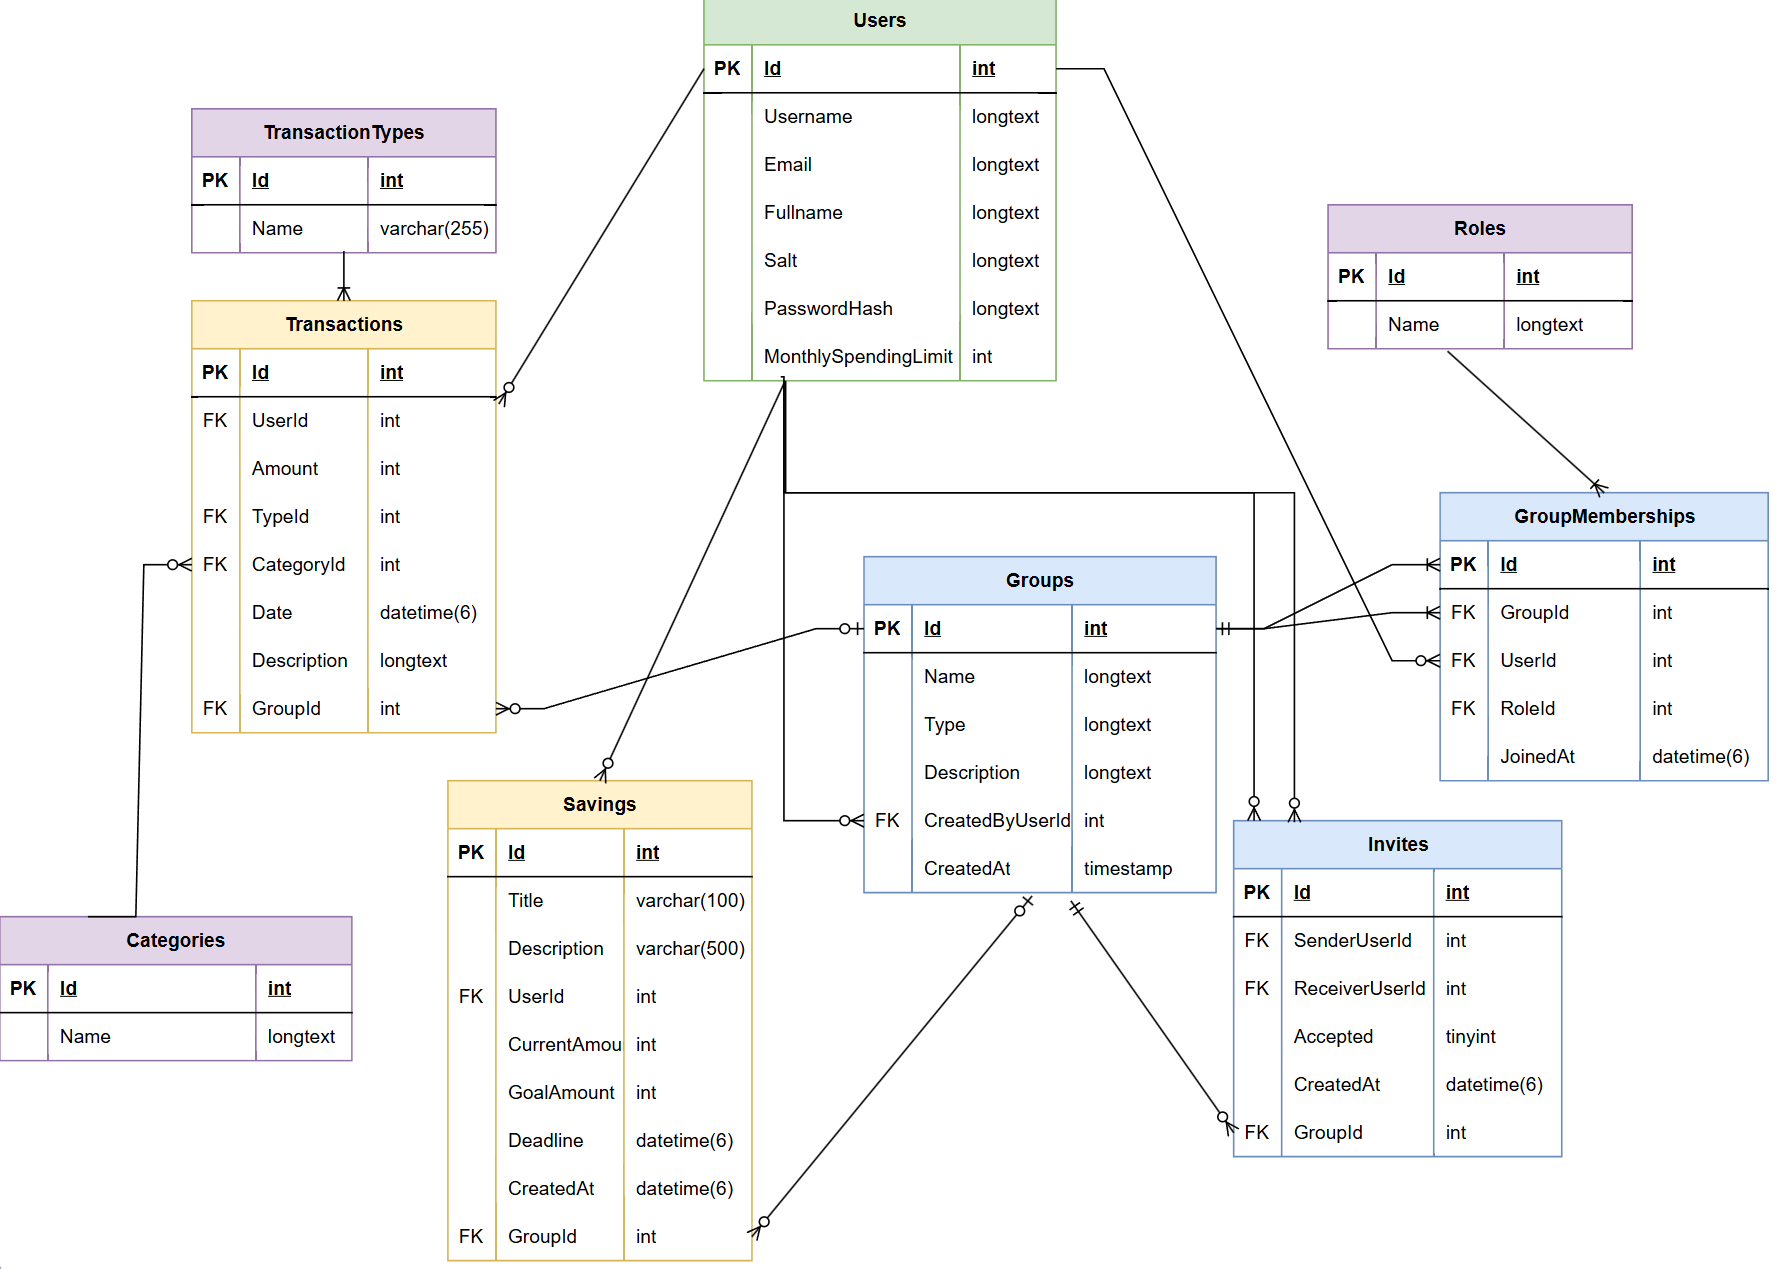
\includegraphics[height=320px]{img/0000}
	\caption{Adatbázis struktúra}
	\label{fig:database-structure}
\end{figure}

\begin{longtable}{ | m{0.25\textwidth} | m{0.65\textwidth} | }
	\hline
	\textbf{Tábla} & \textbf{Leírás} \\
	\hline
	\endfirsthead
	
	\hline
	\textbf{Tábla} & \textbf{Leírás} \\
	\hline
	\endhead
	
	\hline
	\endfoot
	
	\hline
	\caption{Adatbázis táblák magyarázata} \label{tab:db-desc} \\
	\endlastfoot
	
	Users & A rendszer felhasználóit tartalmazza. Itt tároljuk az alapvető adatokat (felhasználónév, e-mail, teljes név), a hitelesítéshez szükséges információkat (salt és jelszóhash), valamint a havi költési limitet is. \\
	\hline
	Groups & A csoportokat kezeli, amelyekbe a felhasználók beléphetnek. Minden csoportnak van neve, típusa (pl. család, baráti társaság, ez szabad szöveges érték), leírása, létrehozó felhasználója és létrehozási dátuma. \\
	\hline
	GroupMemberships & A felhasználók csoporttagságait rögzíti. Megmutatja, hogy ki melyik csoporthoz tartozik, milyen szerepkörben (pl. admin vagy tag), és mióta tagja a csoportnak. \\
	\hline
	Roles & Az egyes csoporttagságokhoz rendelhető szerepköröket definiálja, például adminisztrátor vagy sima tag. A szerepkörök szabályozzák a felhasználók jogosultságait a csoportban. A csoport létrehozójának "Admin" jogköre lesz automatikusan, a felvett tagnak pedig "Member".\\
	\hline
	Transactions & A felhasználók által rögzített pénzügyi tranzakciókat tárolja. Minden tranzakcióhoz tartozik összeg, típus (bevétel vagy kiadás), kategória (pl. étel, szórakozás), dátum, leírás, és adott esetben kapcsolódó csoport is. A "GroupId" értéke null, ha személyes a tranzakció. \\
	\hline
	TransactionTypes & A tranzakciók típusait (bevétel, kiadás) határozza meg. \\
	\hline
	Categories & A tranzakciókhoz tartozó kategóriákat tartalmazza, mint például élelmiszer, közlekedés, szórakozás stb. Segíti a kiadások és bevételek részletesebb elemzését. \\
	\hline
	Savings & A felhasználók által kitűzött megtakarítási célokat tárolja. A célösszeg és a határidő opcionális adatok, tehát lehet null értékük. A "GroupId" értéke is null, ha személyes megtakarítás. \\
	\hline
	Invites & A csoportokba történő meghívásokat kezeli. Menti, hogy ki küldött meghívót kinek, melyik csoportba, és hogy a meghívás elfogadásra került-e. Az elfogadott meghívók "Accepted" értéke 1-re vált a default 0-ról. Elutasítás esetén a meghívó törlődik a táblából. \\
\end{longtable}

\subsection{Backend - Adatbázis kapcsolat}
A backend és az adatbázis közötti kapcsolat kialakítása az ASP.NET keretrendszerben viszonylag egyszerűen megvalósítható. Ehhez elegendő a szükséges NuGet csomagok – például az Entity Framework Core és a MySQL Connector – telepítése. Az adatbázishoz való csatlakozáshoz mindössze egy kapcsolati karakterláncot (connection string) kell megadni az appsettings.json konfigurációs fájlban, amely tartalmazza a szerver nevét, az adatbázis elérési adatait és a hitelesítéshez szükséges információkat.

\lstset{caption={Adatbázis Connection String}, label=src:connstring}
\begin{lstlisting}[language={HTML}]
	"ConnectionStrings": {
		"MySqlConnection": "server=localhost;port=3306;database=betterspend;user=root;password=<<password>>;"
	}
\end{lstlisting}

majd a Program.cs fájlban tudunk ténylegesen csatlakozni:

\lstset{caption={Program.cs: Adatbázis csatlakozás}, label=src:csharp}
\begin{lstlisting}[language={[Sharp]C}]
	// Get MySQL connection string from configuration
	string connectionString = builder.Configuration.GetConnectionString("MySqlConnection");
	
	// Add DB Context to the application
	builder.Services.AddDbContext<ApplicationDbContext>(options =>
	{
		options.UseMySql(connectionString, ServerVersion.AutoDetect(connectionString));
	});
\end{lstlisting}

A tényleges adatbázis modellje:

\lstset{caption={Adatbázis modell}, label=src:dbmodel}
\begin{lstlisting}[language={[Sharp]C}]
using WebApplication1.Model;

namespace WebApplication1.Data
{
	public class ApplicationDbContext : DbContext
	{
		public ApplicationDbContext(DbContextOptions<ApplicationDbContext> options)
		: base(options)
		{
		}
		
		public DbSet<User> Users { get; set; }
		public DbSet<Transaction> Transactions { get; set; }
		public DbSet<Category> Categories { get; set; }
		public DbSet<Role> Roles { get; set; }
		public DbSet<GroupMembership> GroupMemberships { get; set; }
		public DbSet<Group> Groups { get; set; }
		public DbSet<Invite> Invites { get; set; }
		public DbSet<Saving> Savings { get; set; }
		public DbSet<TransactionType> TransactionTypes { get; set; }
		
	}
}
\end{lstlisting}

A kapcsolat létrehozása után az adatbázis teljes mértékben integrálódik az alkalmazáshoz. Az  Entity Framework lehetővé teszi, hogy ne közvetlenül SQL lekérdezésekkel vagy parancsokkal dolgozzunk, hanem a modell osztályokon keresztül, objektumorientált módon kezeljük az adatokat. Ezek az osztályok (pl. User, Transaction) reprezentálják az adatbázis tábláit, és LINQ segítségével egyszerűen végezhetünk lekérdezéseket és módosításokat. A keretrendszer gondoskodik arról, hogy ezek a módosítások automatikusan szinkronizálódjanak az adatbázissal.

\subsection{Migrációk kezelése}

Az alkalmazás későbbi bővítései és karbantartása során az adatbázis szerkezetének módosítása elkerülhetetlen. Ennek biztonságos és nyomon követhető megvalósításához az Entity Framework Core által biztosított migrációs rendszert alkalmaztam. A migrációk segítségével az adatmodell változásai szinkronban tarthatók az adatbázis szerkezetével, miközben lehetőség nyílik a változtatások verziókövetésére is. A működésének lényege, hogy ha módosítást végzünk az egyik adatbázistáblának megfelelő modell osztályban (például új mezőt adunk hozzá vagy megváltoztatjuk egy meglévő típusát vagy akár egy teljesen új modellt hozunk létre), akkor a migrációs rendszer segítségével ez a változás automatikusan átvezethető az adatbázis szerkezetébe is.

Egy új migráció létrehozása a következő paranccsal történik:

\texttt{>>dotnet ef migrations add <Név>}

A migráció alkalmazása az adatbázisra pedig a következő parancs segítségével történik:

\texttt{>>dotnet ef database update}

(vagy A Visual Studio Package Manager Console-ján belül:
"Add-Migration <Név>"
és
"Update-Database"
)

Ez a megközelítés biztosítja, hogy a különböző fejlesztési vagy éles környezetekben is konzisztens adatbázis-struktúra álljon rendelkezésre.

\section{Tesztek}
\begin{table}[h!]
	\centering
	\begin{tabular}{|l|p{10cm}|}
		\hline
		\textbf{Teszteset azonosító} & TC001 \\ \hline
		\textbf{Funkció} & Regisztráció \\ \hline
		\textbf{Bemenet} & Valid e-mail cím, egyedi felhasználónév, teljes név, jelszó \\ \hline
		\textbf{Elvárt eredmény} & Sikeres regisztráció, átirányítás a bejelentkezés felületre, visszajelző üzenet a felhasználónak \\ \hline
		\textbf{Tényleges eredmény} & Megfelel az elvárt eredménynek\\ \hline
	\end{tabular}
	\caption{Sikeres regisztráció}
	\label{tab:manual_testcase_registration}
\end{table}
\begin{table}[h!]
	\centering
	\begin{tabular}{|l|p{10cm}|}
		\hline
		\textbf{Teszteset azonosító} & TC002 \\ \hline
		\textbf{Funkció} & Regisztráció \\ \hline
		\textbf{Bemenet} & Üres mezők beküldése vagy invalid e-mail cím, vagy nem elég erős jelszó \\ \hline
		\textbf{Elvárt eredmény} & Hibajelzés, regisztráció sikertelen \\ \hline
		\textbf{Tényleges eredmény} & Megfelel az elvárt eredménynek \\ \hline
	\end{tabular}
	\caption{Sikertelen regisztráció}
	\label{tab:regisztracio_ures}
\end{table}

\begin{table}[h!]
	\centering
	\begin{tabular}{|l|p{10cm}|}
		\hline
		\textbf{Teszteset azonosító} & TC003 \\ \hline
		\textbf{Funkció} & Bejelentkezés \\ \hline
		\textbf{Bemenet} & Helyes felhasználónév - jelszó páros megadása \\ \hline
		\textbf{Elvárt eredmény} & Belépteti a felhasználót az oldalra \\ \hline
		\textbf{Tényleges eredmény} & Megfelel az elvárt eredménynek \\ \hline
	\end{tabular}
	\caption{Sikeres bejelentkezés}
	\label{tab:bejelentkezes_hibas_adatokkal}
\end{table}

\begin{table}[h!]
	\centering
	\begin{tabular}{|l|p{10cm}|}
		\hline
		\textbf{Teszteset azonosító} & TC004 \\ \hline
		\textbf{Funkció} & Bejelentkezés \\ \hline
		\textbf{Bemenet} & Üres mezők beküldése, vagy helytelen felhasználónév-jelszó páros \\ \hline
		\textbf{Elvárt eredmény} & Hibajelzés, a bejelentkezés sikertelen\\ \hline
		\textbf{Tényleges eredmény} & Megfelel az elvárt eredménynek \\ \hline
	\end{tabular}
	\caption{Sikertelen bejelentkezés}
	\label{tab:bejelentkezes_ures}
\end{table}

\begin{table}[h!]
	\centering
	\begin{tabular}{|l|p{10cm}|}
		\hline
		\textbf{Teszteset azonosító} & TC005 \\ \hline
		\textbf{Funkció} & Profil oldal - adatok módosítása \\ \hline
		\textbf{Bemenet} & Új, egyedi felhasználónév megadása VAGY új, valid e-mail cím megadása VAGY új teljes név megadása \\ \hline
		\textbf{Elvárt eredmény} & Sikeres módosítás \\ \hline
		\textbf{Tényleges eredmény} & Megfelel az elvárt eredménynek \\ \hline
	\end{tabular}
	\caption{Személyes adatok sikeres módosítása}
	\label{tab:profil_felhasznalonev_modositas}
\end{table}

\begin{table}[h!]
	\centering
	\begin{tabular}{|l|p{10cm}|}
		\hline
		\textbf{Teszteset azonosító} & TC006 \\ \hline
		\textbf{Funkció} & Profil oldal - adatok módosítása \\ \hline
		\textbf{Bemenet} & Helytelen e-mail cím megadás, foglalt felhasználónév megadás, üres mező beküldése \\ \hline
		\textbf{Elvárt eredmény} & Hibajelzés, a módosítás nem lép érvénybe \\ \hline
		\textbf{Tényleges eredmény} & Megfelel az elvárt eredménynek \\ \hline
	\end{tabular}
	\caption{Személyes adatok sikertelen módosítása}
	\label{tab:profil_felhasznalonev_foglalt}
\end{table}


\begin{table}[h!]
	\centering
	\begin{tabular}{|l|p{10cm}|}
		\hline
		\textbf{Teszteset azonosító} & TC007 \\ \hline
		\textbf{Funkció} & Profil oldal - Jelszó módosítása \\ \hline
		\textbf{Bemenet} & Helyes régi jelszó, új jelszó, új jelszó megerősítése egyezően, új jelsző elég erős \\ \hline
		\textbf{Elvárt eredmény} & Sikeres jelszóváltás, visszajelzés a felhasználónak \\ \hline
		\textbf{Tényleges eredmény} & Megfelel az elvárt eredménynek \\ \hline
	\end{tabular}
	\caption{Sikeres jelszó modósítás}
	\label{tab:profil_jelszo_modositas}
\end{table}

\begin{table}[h!]
	\centering
	\begin{tabular}{|l|p{10cm}|}
		\hline
		\textbf{Teszteset azonosító} & TC008 \\ \hline
		\textbf{Funkció} & Profil oldal - Jelszó módosítása \\ \hline
		\textbf{Bemenet} & Helytelen régi jelszó, új jelszó és megerősítés nem egyező, nem elég erős új jelszó \\ \hline
		\textbf{Elvárt eredmény} & Hibajelzés, módosítás nem lép érvénybe \\ \hline
		\textbf{Tényleges eredmény} & Megfelel az elvárt eredménynek \\ \hline
	\end{tabular}
	\caption{Sikertelen jelszó módosítás}
	\label{tab:jelszo_modositas_rossz_regi}
\end{table}

\begin{table}[h!]
	\centering
	\begin{tabular}{|l|p{10cm}|}
		\hline
		\textbf{Teszteset azonosító} & TC009 \\ \hline
		\textbf{Funkció} & Új bevétel rögzítése \\ \hline
		\textbf{Bemenet} & Helyes amount (pl. 5000) és description (pl. "Fizetés") \\ \hline
		\textbf{Elvárt eredmény} & Sikeres mentés, üzenet: "Transaction saved!" \\ \hline
		\textbf{Tényleges eredmény} & Megfelel az elvárt eredménynek \\ \hline
	\end{tabular}
	\caption{Új bevétel helyes adatokkal}
	\label{tab:uj_bevetel_helyes}
\end{table}

\begin{table}[h!]
	\centering
	\begin{tabular}{|l|p{10cm}|}
		\hline
		\textbf{Teszteset azonosító} & TC010 \\ \hline
		\textbf{Funkció} & Új bevétel rögzítése \\ \hline
		\textbf{Bemenet} & Üres vagy hibás amount/description mezők \\ \hline
		\textbf{Elvárt eredmény} & Hibajelzés: "Failed to create transaction!" (Tranzakció mentése sikertelen.) \\ \hline
		\textbf{Tényleges eredmény} & Megfelel az elvárt eredménynek \\ \hline
	\end{tabular}
	\caption{Új bevétel hibás adatokkal}
	\label{tab:uj_bevetel_hibas}
\end{table}

\begin{table}[h!]
	\centering
	\begin{tabular}{|l|p{10cm}|}
		\hline
		\textbf{Teszteset azonosító} & TC011 \\ \hline
		\textbf{Funkció} & Kiadás rögzítése, ha havi limit = 0 \\ \hline
		\textbf{Bemenet} & Új kiadás mentése 0 költési limit mellett \\ \hline
		\textbf{Elvárt eredmény} & Üzenet: "Transaction saved!" (limit státusz nélkül) \\ \hline
		\textbf{Tényleges eredmény} & Megfelel az elvárt eredménynek \\ \hline
	\end{tabular}
	\caption{Kiadás rögzítése havi limit nélkül}
	\label{tab:kiadas_limit_nelkul}
\end{table}

\begin{table}[h!]
	\centering
	\begin{tabular}{|l|p{10cm}|}
		\hline
		\textbf{Teszteset azonosító} & TC012 \\ \hline
		\textbf{Funkció} & Kiadás rögzítése, ha van havi limit \\ \hline
		\textbf{Bemenet} & Új kiadás mentése havi limit mellett \\ \hline
		\textbf{Elvárt eredmény} & Limit státusz megjelenik: zöld (ha van keret), sárga (ha túllépés történt) \\ \hline
		\textbf{Tényleges eredmény} & Megfelel az elvárt eredménynek \\ \hline
	\end{tabular}
	\caption{Kiadás rögzítése havi limittel}
	\label{tab:kiadas_limit_ellenorzes}
\end{table}

\begin{table}[h!]
	\centering
	\begin{tabular}{|l|p{10cm}|}
		\hline
		\textbf{Teszteset azonosító} & TC013 \\ \hline
		\textbf{Funkció} & Előzmény táblázat ellenőrzése \\ \hline
		\textbf{Bemenet} & Új bevétel/kiadás rögzítése \\ \hline
		\textbf{Elvárt eredmény} & Az új tranzakció megjelenik az előzmények között \\ \hline
		\textbf{Tényleges eredmény} & Megfelel az elvárt eredménynek \\ \hline
	\end{tabular}
	\caption{Új tranzakció megjelenése az előzmények között}
	\label{tab:elozmeny_tabla}
\end{table}

\begin{table}[h!]
	\centering
	\begin{tabular}{|l|p{10cm}|}
		\hline
		\textbf{Teszteset azonosító} & TC014 \\ \hline
		\textbf{Funkció} & CSV batch feltöltés \\ \hline
		\textbf{Bemenet} & Helyes formátumú CSV fájl feltöltése (típus, kategória, leírás, összeg, dátum) \\ \hline
		\textbf{Elvárt eredmény} & Minden sor külön tranzakcióként mentésre kerül, üzenet: "Transactions saved!" (Tranzakciók elmentve!) \\ \hline
		\textbf{Tényleges eredmény} & Megfelel az elvárt eredménynek \\ \hline
	\end{tabular}
	\caption{CSV batch feltöltés helyes fájllal}
	\label{tab:csv_feltoltes}
\end{table}

\begin{table}[h!]
	\centering
	\begin{tabular}{|l|p{10cm}|}
		\hline
		\textbf{Teszteset azonosító} & TC015 \\ \hline
		\textbf{Funkció} & CSV batch feltöltés \\ \hline
		\textbf{Bemenet} & Helytelen formátumú CSV fájl feltöltése (típus, kategória, leírás, összeg, dátum) \\ \hline
		\textbf{Elvárt eredmény} & Hibaüzenet: "Error! <<a pontos hiba>>" (Hiba!) \\ \hline
		\textbf{Tényleges eredmény} & Megfelel az elvárt eredménynek \\ \hline
	\end{tabular}
	\caption{CSV batch feltöltés helytelen fájllal}
	\label{tab:csv_feltoltes_helytelen}
\end{table}

\begin{table}[h!]
	\centering
	\begin{tabular}{|l|p{10cm}|}
		\hline
		\textbf{Teszteset azonosító} & TC016 \\ \hline
		\textbf{Funkció} & Havi költési limit módosítása \\ \hline
		\textbf{Bemenet} & Új poitív egész költési limit megadása (pl. 100000) \\ \hline
		\textbf{Elvárt eredmény} & Sikeres módosítás, limit frissítése az adatbázisban \\ \hline
		\textbf{Tényleges eredmény} & Megfelel az elvárt eredménynek \\ \hline
	\end{tabular}
	\caption{Sikeres havi költési limit módosítása}
	\label{tab:havi_limit_modositas}
\end{table}
\begin{table}[h!]
	\centering
	\begin{tabular}{|l|p{10cm}|}
		\hline
		\textbf{Teszteset azonosító} & TC017 \\ \hline
		\textbf{Funkció} & Havi költési limit módosítása \\ \hline
		\textbf{Bemenet} & Érvénytelen költési limit megadása (pl. negatív szám)\\ \hline
		\textbf{Elvárt eredmény} & Sikertelen módosítás \\ \hline
		\textbf{Tényleges eredmény} & Megfelel az elvárt eredménynek \\ \hline
	\end{tabular}
	\caption{Sikertelen havi költési limit módosítása}
	\label{tab:havi_limit_modositas_sikertelen}
\end{table}

\begin{table}[h!]
	\centering
	\begin{tabular}{|l|p{10cm}|}
		\hline
		\textbf{Teszteset azonosító} & TC018 \\ \hline
		\textbf{Funkció} & Új megtakarítás létrehozása helyes adatok megadásával \\ \hline
		\textbf{Bemenet} & Név, leírás, célösszeg (opcionális), határidő megadása (opcionális) \\ \hline
		\textbf{Elvárt eredmény} & Sikeres megtakarítás létrejötte a megadott adatokkal \\ \hline
		\textbf{Tényleges eredmény} & Megfelel az elvárt eredménynek \\ \hline
	\end{tabular}
	\caption{Új megtakarítás létrehozása}
	\label{tab:megtakaritas}
\end{table}

\begin{table}[h!]
	\centering
	\begin{tabular}{|l|p{10cm}|}
		\hline
		\textbf{Teszteset azonosító} & TC019 \\ \hline
		\textbf{Funkció} & Összeg hozzáadása megtakarításhoz \\ \hline
		\textbf{Bemenet} & Megtakarításhoz adott összeg megadása (pl. 10000) \\ \hline
		\textbf{Elvárt eredmény} & Az összeg hozzáadódik a megtakarításhoz, frissül az aktuális összeg \\ \hline
		\textbf{Tényleges eredmény} & Megfelel az elvárt eredménynek \\ \hline
	\end{tabular}
	\caption{Összeg hozzáadása megtakarításhoz}
	\label{tab:hozzaadas_megtakaritashoz}
\end{table}

\begin{table}[h!]
	\centering
	\begin{tabular}{|l|p{10cm}|}
		\hline
		\textbf{Teszteset azonosító} & TC020 \\ \hline
		\textbf{Funkció} & Összeg elvétele megtakarításból \\ \hline
		\textbf{Bemenet} & Megtakarításból elvont összeg megadása (pl. 5000) \\ \hline
		\textbf{Elvárt eredmény} & Az összeg levonásra kerül, frissül az aktuális összeg \\ \hline
		\textbf{Tényleges eredmény} & Megfelel az elvárt eredménynek \\ \hline
	\end{tabular}
	\caption{Összeg elvétele megtakarításból}
	\label{tab:elvetel_megtakaritasbol}
\end{table}

\begin{table}[h!]
	\centering
	\begin{tabular}{|l|p{10cm}|}
		\hline
		\textbf{Teszteset azonosító} & TC021 \\ \hline
		\textbf{Funkció} & Megtakarítás törlése \\ \hline
		\textbf{Bemenet} & Meglévő megtakarítás kártyán lévő kuka ikon megnyomása és a törlés megerősítése \\ \hline
		\textbf{Elvárt eredmény} & A kiválasztott megtakarítás törlésre kerül \\ \hline
		\textbf{Tényleges eredmény} & Megfelel az elvárt eredménynek \\ \hline
	\end{tabular}
	\caption{Megtakarítás törlése}
	\label{tab:megtakaritas_torles}
\end{table}

\begin{table}[h!]
	\centering
	\begin{tabular}{|l|p{10cm}|}
		\hline
		\textbf{Teszteset azonosító} & TC022 \\ \hline
		\textbf{Funkció} & Részletes riport letöltése \\ \hline
		\textbf{Bemenet} & Letöltés gombra \\ \hline
		\textbf{Elvárt eredmény} & A részletes riport fájl letöltésre kerül \\ \hline
		\textbf{Tényleges eredmény} & Megfelel az elvárt eredménynek \\ \hline
	\end{tabular}
	\caption{Részletes riport letöltése}
	\label{tab:reszletes_riport_letoltes}
\end{table}

\begin{table}[h!]
	\centering
	\begin{tabular}{|l|p{10cm}|}
		\hline
		\textbf{Teszteset azonosító} & TC023 \\ \hline
		\textbf{Funkció} & Év váltása az éves összefoglaló riporton \\ \hline
		\textbf{Bemenet} & Másik év kiválasztása az éves riport nézetben \\ \hline
		\textbf{Elvárt eredmény} & Az adott évre vonatkozó adatok jelennek meg \\ \hline
		\textbf{Tényleges eredmény} & Megfelel az elvárt eredménynek \\ \hline
	\end{tabular}
	\caption{Év váltása éves összefoglaló riporton}
	\label{tab:ev_valtasa_osszegzo_riport}
\end{table}

\begin{table}[h!]
	\centering
	\begin{tabular}{|l|p{10cm}|}
		\hline
		\textbf{Teszteset azonosító} & TC024 \\ \hline
		\textbf{Funkció} & Új csoport létrehozása \\ \hline
		\textbf{Bemenet} & Csoportnév, típus, leírás megadása, létrehozás gomb megnyomása \\ \hline
		\textbf{Elvárt eredmény} & A csoport sikeresen létrejön és megjelenik a listában \\ \hline
		\textbf{Tényleges eredmény} & Megfelel az elvárt eredménynek \\ \hline
	\end{tabular}
	\caption{Új csoport létrehozása}
	\label{tab:csoport_letrehozas}
\end{table}

\begin{table}[h!]
	\centering
	\begin{tabular}{|l|p{10cm}|}
		\hline
		\textbf{Teszteset azonosító} & TC025 \\ \hline
		\textbf{Funkció} & Csoport törlése \\ \hline
		\textbf{Bemenet} & Meglévő csoport törlésének megerősítése \\ \hline
		\textbf{Elvárt eredmény} & A kiválasztott csoport törlésre kerül a listából \\ \hline
		\textbf{Tényleges eredmény} & Megfelel az elvárt eredménynek \\ \hline
	\end{tabular}
	\caption{Csoport törlése}
	\label{tab:csoport_torles}
\end{table}

\begin{table}[h!]
	\centering
	\begin{tabular}{|l|p{10cm}|}
		\hline
		\textbf{Teszteset azonosító} & TC026 \\ \hline
		\textbf{Funkció} & Csoportban új tranzakció rögzítése \\ \hline
		\textbf{Bemenet} & Összeg és leírás megadása \\ \hline
		\textbf{Elvárt eredmény} & A tranzakció megjelenik a táblázatban a felhasználó nevével és helyes adatokkal \\ \hline
		\textbf{Tényleges eredmény} & Megfelel az elvárt eredménynek \\ \hline
	\end{tabular}
	\caption{Csoportban tranzakció rögzítése}
	\label{tab:csoport_kiadas_rogzitese}
\end{table}

\begin{table}[h!]
	\centering
	\begin{tabular}{|l|p{10cm}|}
		\hline
		\textbf{Teszteset azonosító} & TC027 \\ \hline
		\textbf{Funkció} & Csoport elhagyása \\ \hline
		\textbf{Bemenet} & Csoportból kilépés megerősítése \\ \hline
		\textbf{Elvárt eredmény} & A felhasználó kikerül a csoportból \\ \hline
		\textbf{Tényleges eredmény} & Megfelel az elvárt eredménynek \\ \hline
	\end{tabular}
	\caption{Csoport elhagyása}
	\label{tab:csoport_elhagyasa}
\end{table}

\begin{table}[h!]
	\centering
	\begin{tabular}{|l|p{10cm}|}
		\hline
		\textbf{Teszteset azonosító} & TC028 \\ \hline
		\textbf{Funkció} & Tag meghívása csoporthoz \\ \hline
		\textbf{Bemenet} & Új tag felhasználónevének megadása, meghívó küldése \\ \hline
		\textbf{Elvárt eredmény} & Meghívó elküldve\\ \hline
		\textbf{Tényleges eredmény} & Megfelel az elvárt eredménynek \\ \hline
	\end{tabular}
	\caption{Tag meghívása csoporthoz - sikeres}
	\label{tab:tag_hozzaadasa}
\end{table}

\begin{table}[h!]
	\centering
	\begin{tabular}{|l|p{10cm}|}
		\hline
		\textbf{Teszteset azonosító} & TC029 \\ \hline
		\textbf{Funkció} & Tag meghívása csoporthoz \\ \hline
		\textbf{Bemenet} & Nem létező felhasználónév, üres mezők megadása \\ \hline
		\textbf{Elvárt eredmény} & Hibajelzés, meghívó nem kerül küldésre\\ \hline
		\textbf{Tényleges eredmény} & Megfelel az elvárt eredménynek \\ \hline
	\end{tabular}
	\caption{Tag meghívása csoporthoz - sikertelen}
	\label{tab:tag_hozzaadasa_sikertelen}
\end{table}

\begin{table}[h!]
	\centering
	\begin{tabular}{|l|p{10cm}|}
		\hline
		\textbf{Teszteset azonosító} & TC030 \\ \hline
		\textbf{Funkció} & Meghívó elfogadása \\ \hline
		\textbf{Bemenet} & Meghívó elfogadása az értesítések fülön \\ \hline
		\textbf{Elvárt eredmény} & A felhasználó bekerül a csoportba \\ \hline
		\textbf{Tényleges eredmény} & Megfelel az elvárt eredménynek \\ \hline
	\end{tabular}
	\caption{Meghívó elfogadása}
	\label{tab:meghivo_elfogadasa}
\end{table}

\begin{table}[h!]
	\centering
	\begin{tabular}{|l|p{10cm}|}
		\hline
		\textbf{Teszteset azonosító} & TC031 \\ \hline
		\textbf{Funkció} & Meghívó elutasítása \\ \hline
		\textbf{Bemenet} & Meghívó elutasítása az értesítések fülön \\ \hline
		\textbf{Elvárt eredmény} & A felhasználó nem kerül be a csoportba, meghívás megszűnik \\ \hline
		\textbf{Tényleges eredmény} & Megfelel az elvárt eredménynek \\ \hline
	\end{tabular}
	\caption{Meghívó elutasítása}
	\label{tab:meghivo_elutasitasa}
\end{table}

\begin{table}[h!]
	\centering
	\begin{tabular}{|l|p{10cm}|}
		\hline
		\textbf{Teszteset azonosító} & TC032 \\ \hline
		\textbf{Funkció} & Csoport megtakarítás hozzáadása \\ \hline
		\textbf{Bemenet} & Új megtakarítás név és cél megadása csoport szinten \\ \hline
		\textbf{Elvárt eredmény} & A csoport megtakarítás létrejön és megjelenik a listában \\ \hline
		\textbf{Tényleges eredmény} & Megfelel az elvárt eredménynek \\ \hline
	\end{tabular}
	\caption{Csoport megtakarítás hozzáadása}
	\label{tab:csoport_megtakaritas_hozzaadas}
\end{table}

\begin{table}[h!]
	\centering
	\begin{tabular}{|l|p{10cm}|}
		\hline
		\textbf{Teszteset azonosító} & TC033 \\ \hline
		\textbf{Funkció} & Összeg elvétele csoport megtakarításból \\ \hline
		\textbf{Bemenet} & Összeg megadása, amely levonásra kerül a csoport megtakarításból \\ \hline
		\textbf{Elvárt eredmény} & Az aktuális összeg csökken a megadott összeggel \\ \hline
		\textbf{Tényleges eredmény} & Megfelel az elvárt eredménynek \\ \hline
	\end{tabular}
	\caption{Összeg elvétele csoport megtakarításból}
	\label{tab:csoport_megtakaritas_elvetel}
\end{table}

\begin{table}[h!]
	\centering
	\begin{tabular}{|l|p{10cm}|}
		\hline
		\textbf{Teszteset azonosító} & TC034 \\ \hline
		\textbf{Funkció} & Összeg berakása csoport megtakarításba \\ \hline
		\textbf{Bemenet} & Összeg megadása, amely hozzáadódik a csoport megtakarításhoz \\ \hline
		\textbf{Elvárt eredmény} & Az aktuális összeg nő a megadott összeggel \\ \hline
		\textbf{Tényleges eredmény} & Megfelel az elvárt eredménynek \\ \hline
	\end{tabular}
	\caption{Összeg berakása csoport megtakarításba}
	\label{tab:csoport_megtakaritas_berakas}
\end{table}
\begin{table}[h!]
	\centering
	\begin{tabular}{|l|p{10cm}|}
		\hline
		\textbf{Teszteset azonosító} & TC035 \\ \hline
		\textbf{Funkció} & Csoport megtakarítás törlése \\ \hline
		\textbf{Bemenet} & Kártya melletti kuka ikonra kattintás \\ \hline
		\textbf{Elvárt eredmény} & A kiválasztott csoport megtakarítás törlődik \\ \hline
		\textbf{Tényleges eredmény} & Megfelel az elvárt eredménynek \\ \hline
	\end{tabular}
	\caption{Csoport megtakarítás törlése}
	\label{tab:csoport_megtakaritas_torles}
\end{table}
\begin{table}[h!]
	\centering
	\begin{tabular}{|l|p{10cm}|}
		\hline
		\textbf{Teszteset azonosító} & TC036 \\ \hline
		\textbf{Funkció} & Kijelentkezés \\ \hline
		\textbf{Bemenet} & Baloldali menüsávban található kijelentkezés gomb megnyomása \\ \hline
		\textbf{Elvárt eredmény} & Munkamenet befejezése, átirányítás a bejelentkező felületre \\ \hline
		\textbf{Tényleges eredmény} & Megfelel az elvárt eredménynek \\ \hline
	\end{tabular}
	\caption{Kijelentkezés}
	\label{tab:kijelentkezes}
\end{table}



\cleardoublepage

\chapter{Összegzés}
\label{ch:sum}

Lorem ipsum dolor sit amet, consectetur adipiscing elit. In eu egestas mauris. Quisque nisl elit, varius in erat eu, dictum commodo lorem. Sed commodo libero et sem laoreet consectetur. Fusce ligula arcu, vestibulum et sodales vel, venenatis at velit. Aliquam erat volutpat. Proin condimentum accumsan velit id hendrerit. Cras egestas arcu quis felis placerat, ut sodales velit malesuada. Maecenas et turpis eu turpis placerat euismod. Maecenas a urna viverra, scelerisque nibh ut, malesuada ex.

Aliquam suscipit dignissim tempor. Praesent tortor libero, feugiat et tellus porttitor, malesuada eleifend felis. Orci varius natoque penatibus et magnis dis parturient montes, nascetur ridiculus mus. Nullam eleifend imperdiet lorem, sit amet imperdiet metus pellentesque vitae. Donec nec ligula urna. Aliquam bibendum tempor diam, sed lacinia eros dapibus id. Donec sed vehicula turpis. Aliquam hendrerit sed nulla vitae convallis. Etiam libero quam, pharetra ac est nec, sodales placerat augue. Praesent eu consequat purus.

\cleardoublepage

\chapter{Továbbfejlesztési lehetőségek}
\label{ch:future}

Egy alkalmazást véleményem szerint gyakorlatilag soha nem lehet teljesen befejezettnek tekinteni. Mindig lehet hova fejleszteni, és mindig lesznek új ötletek hozzá, illetve ha más nem is, újabb technológiák egészen biztosan. És egy programozó is folyamatosan tanul, egyre jobb és jobb termékeket igyekszik kiadni a kezei közül.

Ezen webalkalmazás továbbfejlesztésére számos olyan ötletem van, amelyek megvalósítása már nem esett jelen projekt keretei közé. A következő fejezetben ezeket fogom röviden kifejteni.

\section{Statisztikák}
A "Reports" oldal jelenleg 2 darab egyszerű, összegző diagramot tartalmaz csak, de itt azt gondolom sokkal nagyobb potenciál is lehetne. Akár AI modellekkel előállítani statisztikákat, elemezni a költési trendeket, és ezáltal személyre szabott pénzügyi tanácsadást biztosítani a felhasználónak.

Megjegyezném, hogy AI integráció nélkül is érdemes lenne a statisztika sokszínű eszközeit jobban kihasználni, és az adattengerből hasznos következtetéseket levonni.
\section{Tranzakciók}
A tranzakciók lekövetésére és megjelenítésére is számos jobb módszer lehetne, mint amit én ebben a projektben megvalósítottam. A felhasználónak például jelentősen megkönnyítené a dolgát, ha nem manuálisan kellene bevinnie mindig a kiadásait. Erre nyújthat megoldást egy beépített AI technológia, amely egy lefotózott blokk/számla tartalmát értelmezni tudja, és automatikusan, tételenként, rögzíti az alkalmazásba. Ezen felül még lehetne ismétlődő bevételeket és kiadásokat beállítani (például fizetés, lakbér, stb.), ezzel is csökkentvén a felhasználói beavatkozást.
\section{Csoportok}

A csoportos funkciókban szerintem rengeteg potenciál bújik meg. A közös megtakarítások lehetőséget adnak arra, hogy barátok, családtagok vagy akár munkatársak együtt kezeljék bizonyos pénzügyeiket, megtakarításaikat. Az alap koncepción nem sokat változtatnék, inkább a kivitelezésen és a plusz funkciókon. A csoportos takarékoskodás nemcsak anyagi szempontból lehet hatékonyabb, hanem pszichológiai szempontból is motiváló. Ha mások is részt vesznek benne, az ösztönözheti az embert, hogy ő is kitartóbb legyen. Ehhez kapcsolódhatnak különféle motivációs taktikák, mint például haladási grafikonok, ranglisták, vagy gamification-elemek (jelvények, célkitűzések, stb.).

Illetve a jövőben érdemes lehet olyan funkciókat is beépíteni, mint például a csoportos üzenetküldés és kommentelés, és automatikus értesítések a tagoknak a határidőkről, befizetésekről.

Ez a modul nemcsak a közösségi élményt erősítené, hanem a felhasználók aktivitását és elköteleződését is jelentősen növelhetné.

\section{UI}
A felhasználói élmény szempontjából kiemelten fontos, hogy egy alkalmazás átlátható, letisztult és esztétikus legyen. A modern webes elvárások világában a vanilla HTML, CSS és JavaScript (még Bootstrap-tel kiegészítve is) már nem feltétlenül elegendő ahhoz, hogy igazán igényes, vizuálisan is kiemelkedő felhasználói felületet hozzunk létre. Emellett például egy React vagy más frontend keretrendszer alkalmazása nemcsak látványosabb UI-t tesz lehetővé, de strukturáltabb, könnyebben karbantartható kódot is eredményez. Ezért érdemes lehet a felhasználói felületet (UI\footnote{UI = User Interface (felhasználói felület)}) egy modern frameworkben újraalkotni.
\cleardoublepage

% Acknowledgements (optional) - in case your thesis received funding or would like to express special thanks to someone
%\chapter*{\acklabel}
%\addcontentsline{toc}{chapter}{\acklabel}
%---

% Appendices (optional) - useful for detailed information in long tables, many and/or large figures, etc.
%\appendix
%\chapter{Szimulációs eredmények}
\label{appx:simulation}

Lorem ipsum dolor sit amet, consectetur adipiscing elit. Pellentesque facilisis in nibh auctor molestie. Donec porta tortor mauris. Cras in lacus in purus ultricies blandit. Proin dolor erat, pulvinar posuere orci ac, eleifend ultrices libero. Donec elementum et elit a ullamcorper. Nunc tincidunt, lorem et consectetur tincidunt, ante sapien scelerisque neque, eu bibendum felis augue non est. Maecenas nibh arcu, ultrices et libero id, egestas tempus mauris. Etiam iaculis dui nec augue venenatis, fermentum posuere justo congue. Nullam sit amet porttitor sem, at porttitor augue. Proin bibendum justo at ornare efficitur. Donec tempor turpis ligula, vitae viverra felis finibus eu. Curabitur sed libero ac urna condimentum gravida. Donec tincidunt neque sit amet neque luctus auctor vel eget tortor. Integer dignissim, urna ut lobortis volutpat, justo nunc convallis diam, sit amet vulputate erat eros eu velit. Mauris porttitor dictum ante, commodo facilisis ex suscipit sed.

Sed egestas dapibus nisl, vitae fringilla justo. Donec eget condimentum lectus, molestie mattis nunc. Nulla ac faucibus dui. Nullam a congue erat. Ut accumsan sed sapien quis porttitor. Ut pellentesque, est ac posuere pulvinar, tortor mauris fermentum nulla, sit amet fringilla sapien sapien quis velit. Integer accumsan placerat lorem, eu aliquam urna consectetur eget. In ligula orci, dignissim sed consequat ac, porta at metus. Phasellus ipsum tellus, molestie ut lacus tempus, rutrum convallis elit. Suspendisse arcu orci, luctus vitae ultricies quis, bibendum sed elit. Vivamus at sem maximus leo placerat gravida semper vel mi. Etiam hendrerit sed massa ut lacinia. Morbi varius libero odio, sit amet auctor nunc interdum sit amet.

Aenean non mauris accumsan, rutrum nisi non, porttitor enim. Maecenas vel tortor ex. Proin vulputate tellus luctus egestas fermentum. In nec lobortis risus, sit amet tincidunt purus. Nam id turpis venenatis, vehicula nisl sed, ultricies nibh. Suspendisse in libero nec nisi tempor vestibulum. Integer eu dui congue enim venenatis lobortis. Donec sed elementum nunc. Nulla facilisi. Maecenas cursus id lorem et finibus. Sed fermentum molestie erat, nec tempor lorem facilisis cursus. In vel nulla id orci fringilla facilisis. Cras non bibendum odio, ac vestibulum ex. Donec turpis urna, tincidunt ut mi eu, finibus facilisis lorem. Praesent posuere nisl nec dui accumsan, sed interdum odio malesuada.
%\cleardoublepage

% Bibliography (mandatory)
\phantomsection
\addcontentsline{toc}{chapter}{\biblabel}
\printbibliography[title=\biblabel]
\cleardoublepage

% List of figures (optional) - useful over 3-5 figures
\phantomsection
\addcontentsline{toc}{chapter}{\lstfigurelabel}
\listoffigures
\cleardoublepage

% List of tables (optional) - useful over 3-5 tables
\phantomsection
\addcontentsline{toc}{chapter}{\lsttablelabel}
\listoftables
\cleardoublepage

% List of algorithms (optional) - useful over 3-5 algorithms
%\phantomsection
%\addcontentsline{toc}{chapter}{\lstalgorithmlabel}
%\listofalgorithms
%\cleardoublepage

% List of codes (optional) - useful over 3-5 code samples
\phantomsection
\addcontentsline{toc}{chapter}{\lstcodelabel}
\lstlistoflistings
\cleardoublepage

% List of symbols (optional)
%\printnomenclature

\end{document}
